%% LyX 2.2.3 created this file.  For more info, see http://www.lyx.org/.
%% Do not edit unless you really know what you are doing.
\documentclass[english]{article}
\usepackage[osf]{mathpazo}
\renewcommand{\sfdefault}{lmss}
\renewcommand{\ttdefault}{lmtt}
\usepackage[T1]{fontenc}
\usepackage[latin9]{inputenc}
\usepackage[paperwidth=30cm,paperheight=35cm]{geometry}
\geometry{verbose,tmargin=3cm,bmargin=3cm}
\setlength{\parindent}{0bp}
\usepackage{amsmath}
\usepackage{amssymb}

\makeatletter
%%%%%%%%%%%%%%%%%%%%%%%%%%%%%% User specified LaTeX commands.
\usepackage{tikz}
\usetikzlibrary{matrix,arrows,decorations.pathmorphing}
\usetikzlibrary{shapes.geometric}
\usepackage{tikz-cd}
\usepackage{amsthm}
\theoremstyle{plain}
\newtheorem{theorem}{Theorem}[section]
\newtheorem{lemma}[theorem]{Lemma}
\newtheorem{prop}{Proposition}[section]
\newtheorem*{cor}{Corollary}
\theoremstyle{definition}
\newtheorem{defn}{Definition}[section]
\newtheorem{ex}{Exercise} 
\newtheorem{example}{Example}[section]
\theoremstyle{remark}
\newtheorem*{rem}{Remark}
\newtheorem*{note}{Note}
\newtheorem{case}{Case}
\usepackage{graphicx}
\usepackage{amssymb}
\usepackage{tikz-cd}
\usetikzlibrary{calc,arrows,decorations.pathreplacing}
\tikzset{mydot/.style={circle,fill,inner sep=1.5pt},
commutative diagrams/.cd,
  arrow style=tikz,
  diagrams={>=latex},
}

\usepackage{babel}
\usepackage{hyperref}
\hypersetup{
    colorlinks,
    citecolor=black,
    filecolor=black,
    linkcolor=black,
    urlcolor=black
}
\usepackage{pgfplots}
\usetikzlibrary{decorations.markings}
\pgfplotsset{compat=1.9}

\makeatother

\usepackage{babel}
\begin{document}

\title{Trees}

\maketitle
\begin{defn} A $\textbf{tree}$ $T$ is an undirected graph $G=(V,E)$
in which any two vertices are connected by exactly one path. A $\textbf{rooted tree}$
is a tree in which a special vertex is singled out. This singled out
vertex is called the $\textbf{root}$ $r$. An $\textbf{ordered tree}$
is a rooted tree in which an ordering is specified for the children
of each vertex. This is sometimes called a ``plane tree'' because
an ordering of the children is equivalent to an embedding of the tree
in the plane, with the root at the top and the children of each vertex
lower than that vertex. A $\textbf{planted tree}$ is a rooted tree
whose root has vertex degree $1$. A $\textbf{leaf}$ of a rooted
tree is a vertex, which isn't the root, of vertex degree $1$. \end{defn}

\begin{rem} In the following, when we say the word ``tree'', we
are referring specifically to non-planted ordered trees where each
root-to-leaf path has the same length, and the number of nodes at
distance $i$ from the root must be strictly smaller than the number
of nodes at distance $i+1$, until reaching the leaves. Trees of this
type are called ``Cayley trees''. We use the letters $r$ to denote
the root, $\ell_{i}$ to denote leaves, and $v_{i}$ to denote all
other vertices. We can represent such a tree as in the picture below,
where the root is the node which appears at the very top, and the
leaves of the tree are at the very bottom of the tree. We also do
not draw a black dot where a leaf node is. \end{rem}

\hfill \hfill

\begin{center}\begin{tikzpicture}

\node[label=below:$$] (a1) at (0,0) {};
\node[label=below:$$] (a2) at (1,0) {};
\node[label=below:$$] (a3) at (2,0) {};
\node[label=below:$$] (a4) at (3,0) {};
\node[label=below:$$] (a5) at (4,0) {};
\node[label=below:$$] (a6) at (5,0) {};
\node[label=below:$$] (a7) at (6,0) {};
\node[label=below:$$] (a8) at (7,0) {};

\node[circle, fill=black, inner sep=1.5pt, label=below left:$$] (b1) at (0.5,1) {};
\node[circle, fill=black, inner sep=1.5pt, label=below left:$$] (b2) at (2.5,1) {};
\node[circle, fill=black, inner sep=1.5pt, label=below left:$$] (b3) at (4.5,1) {};
\node[circle, fill=black, inner sep=1.5pt, label=below left:$$] (b4) at (6.5,1) {};

\node[circle, fill=black, inner sep=1.5pt, label=below left:$$] (c1) at (1.5,2) {};
\node[circle, fill=black, inner sep=1.5pt, label=below left:$$] (c2) at (5.5,2) {};

\node[circle, fill=black, inner sep=1.5pt, label=below left:$$] (d1) at (3.5,3) {};

\draw (a1) -- (b1);
\draw (a2) -- (b1);
\draw (a3) -- (b2);
\draw (a4) -- (b2);
\draw (a5) -- (b3);
\draw (a6) -- (b3);
\draw (a7) -- (b4);
\draw (a8) -- (b4);

\draw (b1) -- (c1);
\draw (b2) -- (c1);
\draw (b3) -- (c2);
\draw (b4) -- (c2);

\draw (c1) -- (d1);
\draw (c2) -- (d1);



\end{tikzpicture} \end{center}

\hfill \hfill

Let $T$ be a tree with $n$ leaves. When we embed $T$ in the plane,
we label the leftmost leaf $\ell_{1}$. The leaf directly to the right
of $\ell_{1}$ is labeled $\ell_{2}$, and so on. We also want to
keep track of the $\textbf{gap}$ $g_{i}$ in between the labels $\ell_{i}$
and $\ell_{i+1}$ for each $1\leq i\leq n-1$. Formally, we can define
the gap $g_{i}$ to be $\{\ell_{i},\ell_{i+1}\}$. To clarify these
ideas, we label the leaves and gaps in the tree above:

\begin{center}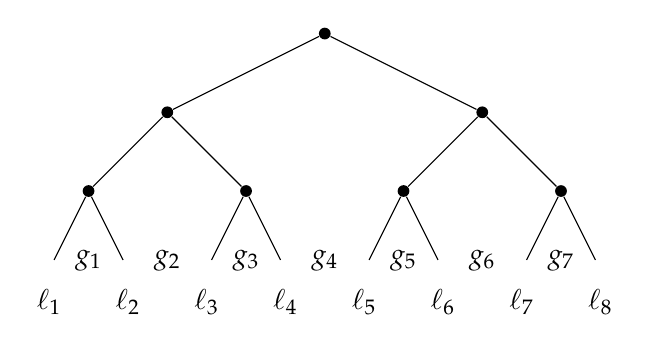
\begin{tikzpicture}

\node[label=below:$ \ell _1 $] (a1) at (0,0) {};
\node[label=below:$ \ell _2 $] (a2) at (1,0) {};
\node[label=below:$ \ell _3 $] (a3) at (2,0) {};
\node[label=below:$ \ell _4 $] (a4) at (3,0) {};
\node[label=below:$ \ell _5 $] (a5) at (4,0) {};
\node[label=below:$ \ell _6 $] (a6) at (5,0) {};
\node[label=below:$ \ell _7 $] (a7) at (6,0) {};
\node[label=below:$ \ell _8 $] (a8) at (7,0) {};

\node[label=below:$ g_1 $] (z1) at (0.5,0.5) {};
\node[label=below:$ g_2 $] (z2) at (1.5,0.5) {};
\node[label=below:$ g_3 $] (z3) at (2.5,0.5) {};
\node[label=below:$ g_4 $] (z4) at (3.5,0.5) {};
\node[label=below:$ g_5 $] (z5) at (4.5,0.5) {};
\node[label=below:$ g_6 $] (z6) at (5.5,0.5) {};
\node[label=below:$ g_7 $] (z7) at (6.5,0.5) {};


\node[circle, fill=black, inner sep=1.5pt, label=below left:$$] (b1) at (0.5,1) {};
\node[circle, fill=black, inner sep=1.5pt, label=below left:$$] (b2) at (2.5,1) {};
\node[circle, fill=black, inner sep=1.5pt, label=below left:$$] (b3) at (4.5,1) {};
\node[circle, fill=black, inner sep=1.5pt, label=below left:$$] (b4) at (6.5,1) {};

\node[circle, fill=black, inner sep=1.5pt, label=below left:$$] (c1) at (1.5,2) {};
\node[circle, fill=black, inner sep=1.5pt, label=below left:$$] (c2) at (5.5,2) {};

\node[circle, fill=black, inner sep=1.5pt, label=below left:$$] (d1) at (3.5,3) {};

\draw (a1) -- (b1);
\draw (a2) -- (b1);
\draw (a3) -- (b2);
\draw (a4) -- (b2);
\draw (a5) -- (b3);
\draw (a6) -- (b3);
\draw (a7) -- (b4);
\draw (a8) -- (b4);

\draw (b1) -- (c1);
\draw (b2) -- (c1);
\draw (b3) -- (c2);
\draw (b4) -- (c2);

\draw (c1) -- (d1);
\draw (c2) -- (d1);



\end{tikzpicture} \end{center}

The gaps may be weakly ordered by the height of their lowest common
ancestor. This weak ordering determines the tree. We write $(x_{11}\cdots x_{1\lambda_{1}})(x_{21}\cdots x_{2\lambda_{2}})\cdots(x_{h1}\cdots x_{h\lambda_{h}})$
where $x_{ij}\in\{1,\dots,n\}$ with $x_{ij}$ are distinct from one
another, $h$ is the height of the tree, and $\lambda_{1}+\cdots+\lambda_{h}=n$,
to mean the tree with $n+1$ leaves such that the gap(s) $g_{x_{11}},\dots,g_{x_{1\lambda_{1}}}$
appear first, the gap(s) $g_{x_{21}},\dots,g_{x_{2\lambda_{2}}}$
to appear second, and so on. Let's go over a few examples to get a
feel for this notation.

\begin{example}The tree below corresponds to $(1357)(26)(5)$

\begin{center}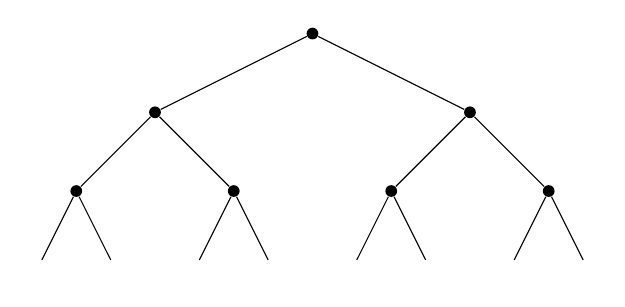
\begin{tikzpicture}

\node[] (a1) at (0,0) {};
\node[] (a2) at (1,0) {};
\node[] (a3) at (2,0) {};
\node[] (a4) at (3,0) {};
\node[] (a5) at (4,0) {};
\node[] (a6) at (5,0) {};
\node[] (a7) at (6,0) {};
\node[] (a8) at (7,0) {};

\node[circle, fill=black, inner sep=1.5pt, label=below left:$$] (b1) at (0.5,1) {};
\node[circle, fill=black, inner sep=1.5pt, label=below left:$$] (b2) at (2.5,1) {};
\node[circle, fill=black, inner sep=1.5pt, label=below left:$$] (b3) at (4.5,1) {};
\node[circle, fill=black, inner sep=1.5pt, label=below left:$$] (b4) at (6.5,1) {};

\node[circle, fill=black, inner sep=1.5pt, label=below left:$$] (c1) at (1.5,2) {};
\node[circle, fill=black, inner sep=1.5pt, label=below left:$$] (c2) at (5.5,2) {};

\node[circle, fill=black, inner sep=1.5pt, label=below left:$$] (d1) at (3.5,3) {};

\draw (a1) -- (b1);
\draw (a2) -- (b1);
\draw (a3) -- (b2);
\draw (a4) -- (b2);
\draw (a5) -- (b3);
\draw (a6) -- (b3);
\draw (a7) -- (b4);
\draw (a8) -- (b4);

\draw (b1) -- (c1);
\draw (b2) -- (c1);
\draw (b3) -- (c2);
\draw (b4) -- (c2);

\draw (c1) -- (d1);
\draw (c2) -- (d1);



\end{tikzpicture} \end{center}

\end{example}

\begin{example}The tree below corresponds to $(1468)(237)(5)$.

\begin{center}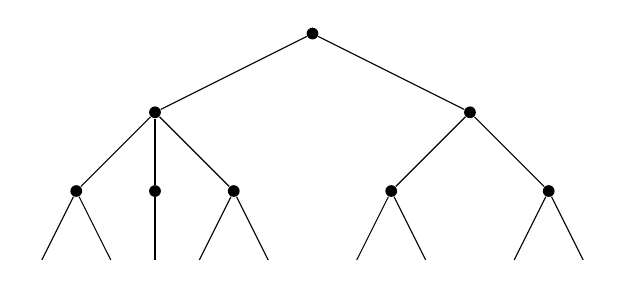
\begin{tikzpicture}

\node[] (a1) at (0,0) {};
\node[] (a2) at (1,0) {};
\node[] (a9) at (1.5,0) {};
\node[] (a3) at (2,0) {};
\node[] (a4) at (3,0) {};
\node[] (a5) at (4,0) {};
\node[] (a6) at (5,0) {};
\node[] (a7) at (6,0) {};
\node[] (a8) at (7,0) {};

\node[circle, fill=black, inner sep=1.5pt, label=below left:$$] (b1) at (0.5,1) {};
\node[circle, fill=black, inner sep=1.5pt, label=below left:$$] (b5) at (1.5,1) {};
\node[circle, fill=black, inner sep=1.5pt, label=below left:$$] (b2) at (2.5,1) {};
\node[circle, fill=black, inner sep=1.5pt, label=below left:$$] (b3) at (4.5,1) {};
\node[circle, fill=black, inner sep=1.5pt, label=below left:$$] (b4) at (6.5,1) {};


\node[circle, fill=black, inner sep=1.5pt, label=below left:$$] (c1) at (1.5,2) {};
\node[circle, fill=black, inner sep=1.5pt, label=below left:$$] (c2) at (5.5,2) {};

\node[circle, fill=black, inner sep=1.5pt, label=below left:$$] (d1) at (3.5,3) {};

\draw (a1) -- (b1);
\draw (a2) -- (b1);
\draw (a9) -- (b5);
\draw (a3) -- (b2);
\draw (a4) -- (b2);
\draw (a5) -- (b3);
\draw (a6) -- (b3);
\draw (a7) -- (b4);
\draw (a8) -- (b4);

\draw (b1) -- (c1);
\draw (b5) -- (c1);
\draw (b2) -- (c1);
\draw (b3) -- (c2);
\draw (b4) -- (c2);

\draw (c1) -- (d1);
\draw (c2) -- (d1);



\end{tikzpicture} \end{center}

\end{example}

\begin{example} The tree below corresponds to $(1)(3)(7)(5)(2)(6)(4)$.

\begin{center}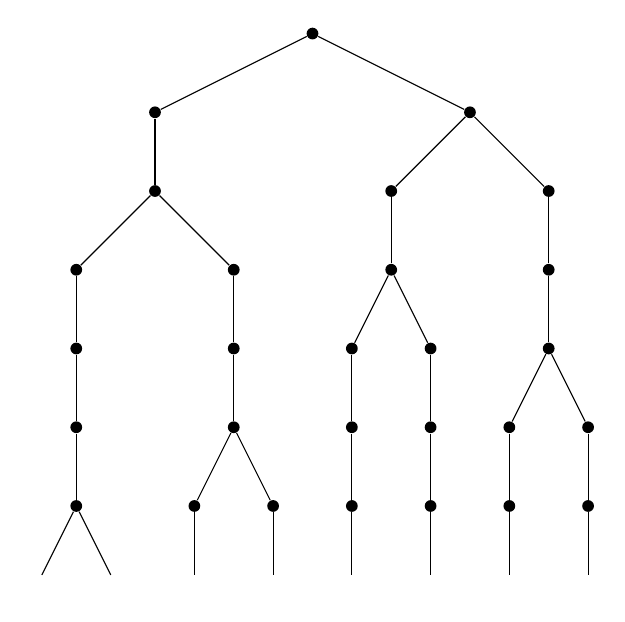
\begin{tikzpicture}

\node[] (a1) at (0,0) {};
\node[] (a2) at (1,0) {};
\node[] (a3) at (2,0) {};
\node[] (a4) at (3,0) {};
\node[] (a5) at (4,0) {};
\node[] (a6) at (5,0) {};
\node[] (a7) at (6,0) {};
\node[] (a8) at (7,0) {};

\node[circle, fill=black, inner sep=1.5pt, label=below left:$$] (b1) at (0.5,1) {};
\node[circle, fill=black, inner sep=1.5pt, label=below left:$$] (b2) at (2,1) {};
\node[circle, fill=black, inner sep=1.5pt, label=below left:$$] (b3) at (3,1) {};
\node[circle, fill=black, inner sep=1.5pt, label=below left:$$] (b4) at (4,1) {};
\node[circle, fill=black, inner sep=1.5pt, label=below left:$$] (b5) at (5,1) {};
\node[circle, fill=black, inner sep=1.5pt, label=below left:$$] (b6) at (6,1) {};
\node[circle, fill=black, inner sep=1.5pt, label=below left:$$] (b7) at (7,1) {};

\node[circle, fill=black, inner sep=1.5pt, label=below left:$$] (c1) at (0.5,2) {};
\node[circle, fill=black, inner sep=1.5pt, label=below left:$$] (c2) at (2.5,2) {};
\node[circle, fill=black, inner sep=1.5pt, label=below left:$$] (c3) at (4,2) {};
\node[circle, fill=black, inner sep=1.5pt, label=below left:$$] (c4) at (5,2) {};
\node[circle, fill=black, inner sep=1.5pt, label=below left:$$] (c5) at (6,2) {};
\node[circle, fill=black, inner sep=1.5pt, label=below left:$$] (c6) at (7,2) {};

\node[circle, fill=black, inner sep=1.5pt, label=below left:$$] (d1) at (0.5,3) {};
\node[circle, fill=black, inner sep=1.5pt, label=below left:$$] (d2) at (2.5,3) {};
\node[circle, fill=black, inner sep=1.5pt, label=below left:$$] (d3) at (4,3) {};
\node[circle, fill=black, inner sep=1.5pt, label=below left:$$] (d4) at (5,3) {};
\node[circle, fill=black, inner sep=1.5pt, label=below left:$$] (d5) at (6.5,3) {};

\node[circle, fill=black, inner sep=1.5pt, label=below left:$$] (e1) at (0.5,4) {};
\node[circle, fill=black, inner sep=1.5pt, label=below left:$$] (e2) at (2.5,4) {};
\node[circle, fill=black, inner sep=1.5pt, label=below left:$$] (e3) at (4.5,4) {};
\node[circle, fill=black, inner sep=1.5pt, label=below left:$$] (e4) at (6.5,4) {};

\node[circle, fill=black, inner sep=1.5pt, label=below left:$$] (f1) at (1.5,5) {};
\node[circle, fill=black, inner sep=1.5pt, label=below left:$$] (f2) at (4.5,5) {};
\node[circle, fill=black, inner sep=1.5pt, label=below left:$$] (f3) at (6.5,5) {};

\node[circle, fill=black, inner sep=1.5pt, label=below left:$$] (g1) at (1.5,6) {};
\node[circle, fill=black, inner sep=1.5pt, label=below left:$$] (g2) at (5.5,6) {};

\node[circle, fill=black, inner sep=1.5pt, label=below left:$$] (h1) at (3.5,7) {};


\draw (a1) -- (b1);
\draw (a2) -- (b1);
\draw (a3) -- (b2);
\draw (a4) -- (b3);
\draw (a5) -- (b4);
\draw (a6) -- (b5);
\draw (a7) -- (b6);
\draw (a8) -- (b7);

\draw (b1) -- (c1);
\draw (b2) -- (c2);
\draw (b3) -- (c2);
\draw (b4) -- (c3);
\draw (b5) -- (c4);
\draw (b6) -- (c5);
\draw (b7) -- (c6);

\draw (c1) -- (d1);
\draw (c2) -- (d2);
\draw (c3) -- (d3);
\draw (c4) -- (d4);
\draw (c5) -- (d5);
\draw (c6) -- (d5);

\draw (d1) -- (e1);
\draw (d2) -- (e2);
\draw (d3) -- (e3);
\draw (d4) -- (e3);
\draw (d5) -- (e4);

\draw (e1) -- (f1);
\draw (e2) -- (f1);
\draw (e3) -- (f2);
\draw (e4) -- (f3);

\draw (f1) -- (g1);
\draw (f2) -- (g2);
\draw (f3) -- (g2);

\draw (g1) -- (h1);
\draw (g2) -- (h1);

\end{tikzpicture} \end{center}

\end{example}

\begin{example} The tree below corresponds to $(13)(7)(5)(2)(6)(4)$.

\begin{center}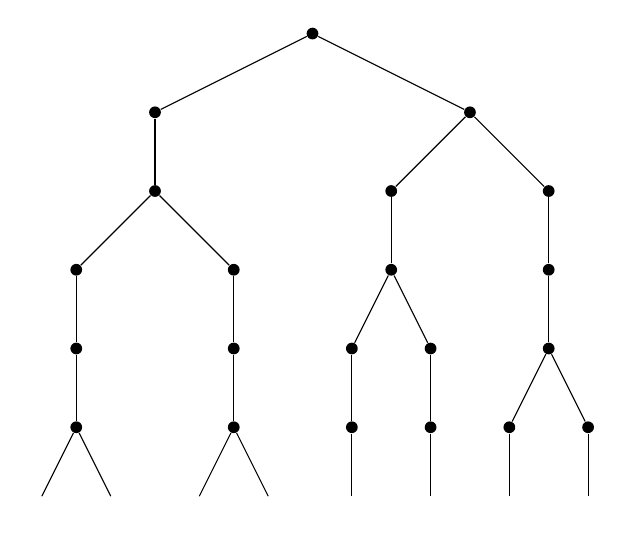
\begin{tikzpicture}

\node[] (b0) at (0,1) {};
\node[] (b1) at (1,1) {};
\node[] (b2) at (2,1) {};
\node[] (b3) at (3,1) {};
\node[] (b4) at (4,1) {};
\node[] (b5) at (5,1) {};
\node[] (b6) at (6,1) {};
\node[] (b7) at (7,1) {};

\node[circle, fill=black, inner sep=1.5pt, label=below left:$$] (c1) at (0.5,2) {};
\node[circle, fill=black, inner sep=1.5pt, label=below left:$$] (c2) at (2.5,2) {};
\node[circle, fill=black, inner sep=1.5pt, label=below left:$$] (c3) at (4,2) {};
\node[circle, fill=black, inner sep=1.5pt, label=below left:$$] (c4) at (5,2) {};
\node[circle, fill=black, inner sep=1.5pt, label=below left:$$] (c5) at (6,2) {};
\node[circle, fill=black, inner sep=1.5pt, label=below left:$$] (c6) at (7,2) {};

\node[circle, fill=black, inner sep=1.5pt, label=below left:$$] (d1) at (0.5,3) {};
\node[circle, fill=black, inner sep=1.5pt, label=below left:$$] (d2) at (2.5,3) {};
\node[circle, fill=black, inner sep=1.5pt, label=below left:$$] (d3) at (4,3) {};
\node[circle, fill=black, inner sep=1.5pt, label=below left:$$] (d4) at (5,3) {};
\node[circle, fill=black, inner sep=1.5pt, label=below left:$$] (d5) at (6.5,3) {};

\node[circle, fill=black, inner sep=1.5pt, label=below left:$$] (e1) at (0.5,4) {};
\node[circle, fill=black, inner sep=1.5pt, label=below left:$$] (e2) at (2.5,4) {};
\node[circle, fill=black, inner sep=1.5pt, label=below left:$$] (e3) at (4.5,4) {};
\node[circle, fill=black, inner sep=1.5pt, label=below left:$$] (e4) at (6.5,4) {};

\node[circle, fill=black, inner sep=1.5pt, label=below left:$$] (f1) at (1.5,5) {};
\node[circle, fill=black, inner sep=1.5pt, label=below left:$$] (f2) at (4.5,5) {};
\node[circle, fill=black, inner sep=1.5pt, label=below left:$$] (f3) at (6.5,5) {};

\node[circle, fill=black, inner sep=1.5pt, label=below left:$$] (g1) at (1.5,6) {};
\node[circle, fill=black, inner sep=1.5pt, label=below left:$$] (g2) at (5.5,6) {};

\node[circle, fill=black, inner sep=1.5pt, label=below left:$$] (h1) at (3.5,7) {};

\draw (b0) -- (c1);
\draw (b1) -- (c1);
\draw (b2) -- (c2);
\draw (b3) -- (c2);
\draw (b4) -- (c3);
\draw (b5) -- (c4);
\draw (b6) -- (c5);
\draw (b7) -- (c6);

\draw (c1) -- (d1);
\draw (c2) -- (d2);
\draw (c3) -- (d3);
\draw (c4) -- (d4);
\draw (c5) -- (d5);
\draw (c6) -- (d5);

\draw (d1) -- (e1);
\draw (d2) -- (e2);
\draw (d3) -- (e3);
\draw (d4) -- (e3);
\draw (d5) -- (e4);

\draw (e1) -- (f1);
\draw (e2) -- (f1);
\draw (e3) -- (f2);
\draw (e4) -- (f3);

\draw (f1) -- (g1);
\draw (f2) -- (g2);
\draw (f3) -- (g2);

\draw (g1) -- (h1);
\draw (g2) -- (h1);

\end{tikzpicture} \end{center}

\end{example}

\begin{example} The tree below corresponds to $(3)(1)(7)(5)(2)(6)(4)$.

\begin{center}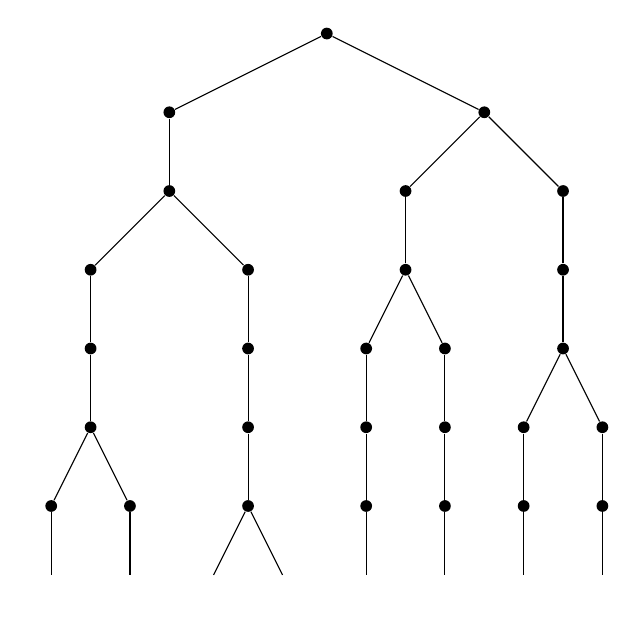
\begin{tikzpicture}

\node[] (a1) at (0,0) {};
\node[] (a2) at (1,0) {};
\node[] (a3) at (2,0) {};
\node[] (a4) at (3,0) {};
\node[] (a5) at (4,0) {};
\node[] (a6) at (5,0) {};
\node[] (a7) at (6,0) {};
\node[] (a8) at (7,0) {};

\node[circle, fill=black, inner sep=1.5pt, label=below left:$$] (b1) at (0,1) {};
\node[circle, fill=black, inner sep=1.5pt, label=below left:$$] (b2) at (1,1) {};
\node[circle, fill=black, inner sep=1.5pt, label=below left:$$] (b3) at (2.5,1) {};
\node[circle, fill=black, inner sep=1.5pt, label=below left:$$] (b4) at (4,1) {};
\node[circle, fill=black, inner sep=1.5pt, label=below left:$$] (b5) at (5,1) {};
\node[circle, fill=black, inner sep=1.5pt, label=below left:$$] (b6) at (6,1) {};
\node[circle, fill=black, inner sep=1.5pt, label=below left:$$] (b7) at (7,1) {};

\node[circle, fill=black, inner sep=1.5pt, label=below left:$$] (c1) at (0.5,2) {};
\node[circle, fill=black, inner sep=1.5pt, label=below left:$$] (c2) at (2.5,2) {};
\node[circle, fill=black, inner sep=1.5pt, label=below left:$$] (c3) at (4,2) {};
\node[circle, fill=black, inner sep=1.5pt, label=below left:$$] (c4) at (5,2) {};
\node[circle, fill=black, inner sep=1.5pt, label=below left:$$] (c5) at (6,2) {};
\node[circle, fill=black, inner sep=1.5pt, label=below left:$$] (c6) at (7,2) {};

\node[circle, fill=black, inner sep=1.5pt, label=below left:$$] (d1) at (0.5,3) {};
\node[circle, fill=black, inner sep=1.5pt, label=below left:$$] (d2) at (2.5,3) {};
\node[circle, fill=black, inner sep=1.5pt, label=below left:$$] (d3) at (4,3) {};
\node[circle, fill=black, inner sep=1.5pt, label=below left:$$] (d4) at (5,3) {};
\node[circle, fill=black, inner sep=1.5pt, label=below left:$$] (d5) at (6.5,3) {};

\node[circle, fill=black, inner sep=1.5pt, label=below left:$$] (e1) at (0.5,4) {};
\node[circle, fill=black, inner sep=1.5pt, label=below left:$$] (e2) at (2.5,4) {};
\node[circle, fill=black, inner sep=1.5pt, label=below left:$$] (e3) at (4.5,4) {};
\node[circle, fill=black, inner sep=1.5pt, label=below left:$$] (e4) at (6.5,4) {};

\node[circle, fill=black, inner sep=1.5pt, label=below left:$$] (f1) at (1.5,5) {};
\node[circle, fill=black, inner sep=1.5pt, label=below left:$$] (f2) at (4.5,5) {};
\node[circle, fill=black, inner sep=1.5pt, label=below left:$$] (f3) at (6.5,5) {};

\node[circle, fill=black, inner sep=1.5pt, label=below left:$$] (g1) at (1.5,6) {};
\node[circle, fill=black, inner sep=1.5pt, label=below left:$$] (g2) at (5.5,6) {};

\node[circle, fill=black, inner sep=1.5pt, label=below left:$$] (h1) at (3.5,7) {};


\draw (a1) -- (b1);
\draw (a2) -- (b2);
\draw (a3) -- (b3);
\draw (a4) -- (b3);
\draw (a5) -- (b4);
\draw (a6) -- (b5);
\draw (a7) -- (b6);
\draw (a8) -- (b7);

\draw (b1) -- (c1);
\draw (b2) -- (c1);
\draw (b3) -- (c2);
\draw (b4) -- (c3);
\draw (b5) -- (c4);
\draw (b6) -- (c5);
\draw (b7) -- (c6);

\draw (c1) -- (d1);
\draw (c2) -- (d2);
\draw (c3) -- (d3);
\draw (c4) -- (d4);
\draw (c5) -- (d5);
\draw (c6) -- (d5);

\draw (d1) -- (e1);
\draw (d2) -- (e2);
\draw (d3) -- (e3);
\draw (d4) -- (e3);
\draw (d5) -- (e4);

\draw (e1) -- (f1);
\draw (e2) -- (f1);
\draw (e3) -- (f2);
\draw (e4) -- (f3);

\draw (f1) -- (g1);
\draw (f2) -- (g2);
\draw (f3) -- (g2);

\draw (g1) -- (h1);
\draw (g2) -- (h1);

\end{tikzpicture} \end{center}

\end{example}

\begin{center}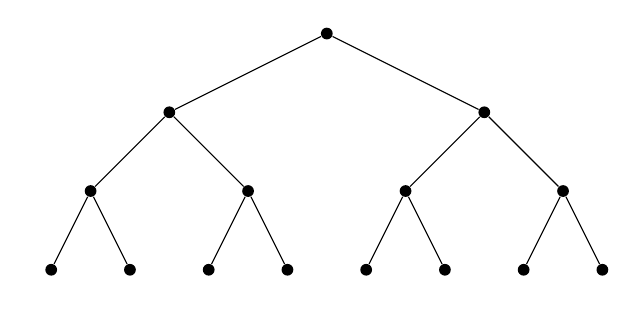
\begin{tikzpicture}

\node[circle, fill=black, inner sep=1.5pt, label=below left:$$] (a1) at (0,0) {};
\node[circle, fill=black, inner sep=1.5pt, label=below left:$$] (a2) at (1,0) {};
\node[circle, fill=black, inner sep=1.5pt, label=below left:$$] (a3) at (2,0) {};
\node[circle, fill=black, inner sep=1.5pt, label=below left:$$] (a4) at (3,0) {};
\node[circle, fill=black, inner sep=1.5pt, label=below left:$$] (a5) at (4,0) {};
\node[circle, fill=black, inner sep=1.5pt, label=below left:$$] (a6) at (5,0) {};
\node[circle, fill=black, inner sep=1.5pt, label=below left:$$] (a7) at (6,0) {};
\node[circle, fill=black, inner sep=1.5pt, label=below left:$$] (a8) at (7,0) {};

\node[circle, fill=black, inner sep=1.5pt, label=below left:$$] (b1) at (0.5,1) {};
\node[circle, fill=black, inner sep=1.5pt, label=below left:$$] (b2) at (2.5,1) {};
\node[circle, fill=black, inner sep=1.5pt, label=below left:$$] (b3) at (4.5,1) {};
\node[circle, fill=black, inner sep=1.5pt, label=below left:$$] (b4) at (6.5,1) {};

\node[circle, fill=black, inner sep=1.5pt, label=below left:$$] (c1) at (1.5,2) {};
\node[circle, fill=black, inner sep=1.5pt, label=below left:$$] (c2) at (5.5,2) {};

\node[circle, fill=black, inner sep=1.5pt, label=below left:$$] (d1) at (3.5,3) {};

\draw (a1) -- (b1);
\draw (a2) -- (b1);
\draw (a3) -- (b2);
\draw (a4) -- (b2);
\draw (a5) -- (b3);
\draw (a6) -- (b3);
\draw (a7) -- (b4);
\draw (a8) -- (b4);

\draw (b1) -- (c1);
\draw (b2) -- (c1);
\draw (b3) -- (c2);
\draw (b4) -- (c2);

\draw (c1) -- (d1);
\draw (c2) -- (d1);



\end{tikzpicture} \end{center}

\begin{center}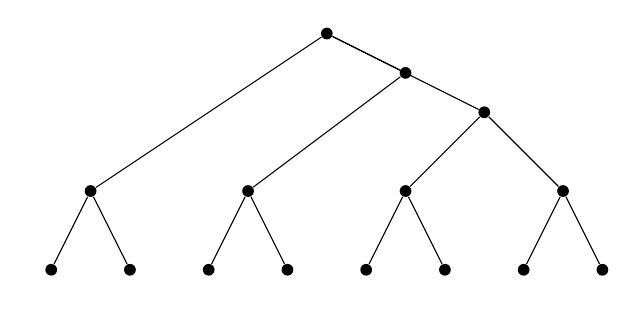
\begin{tikzpicture}

\node[circle, fill=black, inner sep=1.5pt, label=below left:$$] (a1) at (0,0) {};
\node[circle, fill=black, inner sep=1.5pt, label=below left:$$] (a2) at (1,0) {};
\node[circle, fill=black, inner sep=1.5pt, label=below left:$$] (a3) at (2,0) {};
\node[circle, fill=black, inner sep=1.5pt, label=below left:$$] (a4) at (3,0) {};
\node[circle, fill=black, inner sep=1.5pt, label=below left:$$] (a5) at (4,0) {};
\node[circle, fill=black, inner sep=1.5pt, label=below left:$$] (a6) at (5,0) {};
\node[circle, fill=black, inner sep=1.5pt, label=below left:$$] (a7) at (6,0) {};
\node[circle, fill=black, inner sep=1.5pt, label=below left:$$] (a8) at (7,0) {};

\node[circle, fill=black, inner sep=1.5pt, label=below left:$$] (b1) at (0.5,1) {};
\node[circle, fill=black, inner sep=1.5pt, label=below left:$$] (b2) at (2.5,1) {};
\node[circle, fill=black, inner sep=1.5pt, label=below left:$$] (b3) at (4.5,1) {};
\node[circle, fill=black, inner sep=1.5pt, label=below left:$$] (b4) at (6.5,1) {};

\node[circle, fill=black, inner sep=1.5pt, label=below left:$$] (c1) at (4.5,2.5) {};
\node[circle, fill=black, inner sep=1.5pt, label=below left:$$] (c2) at (5.5,2) {};

\node[circle, fill=black, inner sep=1.5pt, label=below left:$$] (d1) at (3.5,3) {};

\draw (a1) -- (b1);
\draw (a2) -- (b1);
\draw (a3) -- (b2);
\draw (a4) -- (b2);
\draw (a5) -- (b3);
\draw (a6) -- (b3);
\draw (a7) -- (b4);
\draw (a8) -- (b4);

\draw (b1) -- (d1);
\draw (b2) -- (c1);
\draw (b3) -- (c2);
\draw (b4) -- (c2);

\draw (c1) -- (d1);
\draw (c2) -- (d1);



\end{tikzpicture} \end{center}

\section*{Permutohedron}

\begin{defn}The $\textbf{permutohedron}$ of order $n$ is an $(n-1)$-dimensional
polytope embedded in an $n$-dimensional space, whose vertices are
formed by permuting the coordinates of the vector $(1,2,3,\dots,n)$.
\end{defn}

\section*{The Permutative Law}

~~~If a mathematical construction generalizes an elementary algebraic
law like associativity or distributivity, then it's bound to be very
useful. We introduce a new type of algebraic law which we call the
\textbf{permutative law} since it corresponds with the permutohedron
as the associative law corresponds with associahedron.

\begin{defn} Let $A$ be a set equipped with a binary operation $\cdot:A\times A\to A$
and a unary operation $f:A\to A$. We say the triple $\mathcal{A}=(A,f,\cdot)$
is \textbf{permutative} when for all $a,b,c,d\in A$, 
\begin{equation}
(f(a)f(b))f(cd)=f(ab)(f(c)f(d))\label{eq:permutativelaw}
\end{equation}

\end{defn}

There's a very nice way of capturing this law in terms of Cayley trees:

\begin{center}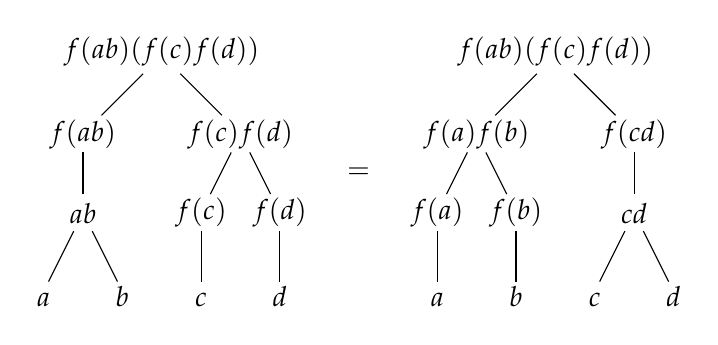
\begin{tikzpicture}

\node[label={[label distance=-0.45cm]90:$a$}] (a1) at (0,0) {};
\node[label={[label distance=-0.45cm]90:$b$}] (a2) at (1,0) {};
\node[label={[label distance=-0.45cm]90:$c$}] (a3) at (2,0) {};
\node[label={[label distance=-0.45cm]90:$d$}] (a4) at (3,0) {};

\node[label={[label distance=-0.5cm]90:$ab$}, inner sep=6.5pt] (b1) at (0.5,1) {};
\node[label={[label distance=-0.55cm]90:$f(c)$}, inner sep=6.5pt] (b2) at (2,1) {};
\node[label={[label distance=-0.55cm]90:$f(d)$}, inner sep=6.5pt] (b3) at (3,1) {};

\node[label={[label distance=-0.55cm]90:$f(ab)$}, inner sep=6.5pt] (c1) at (0.5,2) {};
\node[label={[label distance=-0.55cm]90:$f(c)f(d)$}, inner sep=6.5pt] (c2) at (2.5,2) {};

\node[label={[label distance=-0.5cm]90:$f(ab)(f(c)f(d))$}, inner sep=6.5pt] (d1) at (1.5,3) {};



\draw (a1) -- (b1);
\draw (a2) -- (b1);
\draw (a3) -- (b2);
\draw (a4) -- (b3);

\draw (b1) -- (c1);
\draw (b2) -- (c2);
\draw (b3) -- (c2);

\draw (c1) -- (d1);
\draw (c2) -- (d1);





\node[label={[label distance=-0.45cm]90:$a$}] (aa1) at (5,0) {};
\node[label={[label distance=-0.45cm]90:$b$}] (aa2) at (6,0) {};
\node[label={[label distance=-0.45cm]90:$c$}] (aa3) at (7,0) {};
\node[label={[label distance=-0.45cm]90:$d$}] (aa4) at (8,0) {};

\node[label={[label distance=-0.5cm]90:$cd$}, inner sep=6.5pt] (bb1) at (7.5,1) {};
\node[label={[label distance=-0.55cm]90:$f(a)$}, inner sep=6.5pt] (bb2) at (5,1) {};
\node[label={[label distance=-0.55cm]90:$f(b)$}, inner sep=6.5pt] (bb3) at (6,1) {};

\node[label={[label distance=-0.55cm]90:$f(cd)$}, inner sep=6.5pt] (cc1) at (7.5,2) {};
\node[label={[label distance=-0.55cm]90:$f(a)f(b)$}, inner sep=6.5pt] (cc2) at (5.5,2) {};

\node[label={[label distance=-0.5cm]90:$f(ab)(f(c)f(d))$}, inner sep=6.5pt] (dd1) at (6.5,3) {};



\draw (aa1) -- (bb2);
\draw (aa2) -- (bb3);
\draw (aa3) -- (bb1);
\draw (aa4) -- (bb1);

\draw (bb1) -- (cc1);
\draw (bb2) -- (cc2);
\draw (bb3) -- (cc2);

\draw (cc1) -- (dd1);
\draw (cc2) -- (dd1);

\node[] (x) at (4,1.5) {$=$};

\end{tikzpicture} \end{center}

This is analagous to how we can express the associative law in terms
of binary rooted trees:

\begin{center}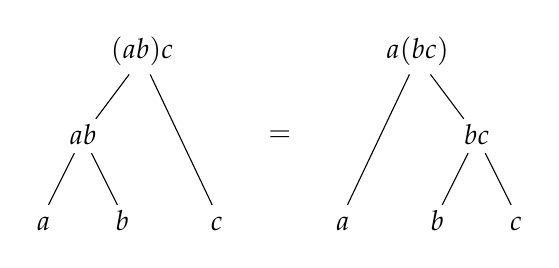
\begin{tikzpicture}

\node[label={[label distance=-0.45cm]90:$a$}] (a1) at (0,0) {};
\node[label={[label distance=-0.45cm]90:$b$}] (a2) at (1,0) {};
\node[label={[label distance=-0.45cm]90:$c$}] (a3) at (2.2,0) {};


\node[label={[label distance=-0.45cm]90:$ab$}, inner sep=6pt] (b1) at (0.5,1) {};

\node[label={[label distance=-0.45cm]90:$(ab)c$}, inner sep=6pt] (c1) at (1.25,2) {};


\draw (a1) -- (b1);
\draw (a2) -- (b1);

\draw (b1) -- (c1);
\draw (a3) -- (c1);


\node[label={[label distance=-0.45cm]90:$a$}] (aa1) at (3.8,0) {};
\node[label={[label distance=-0.45cm]90:$b$}] (aa2) at (5,0) {};
\node[label={[label distance=-0.45cm]90:$c$}] (aa3) at (6,0) {};

\node[label={[label distance=-0.45cm]90:$bc$}, inner sep=6pt] (bb2) at (5.5,1) {};

\node[label={[label distance=-0.45cm]90:$a(bc)$}, inner sep=6pt] (cc1) at (4.75,2) {};

\draw (aa2) -- (bb2);
\draw (aa3) -- (bb2);

\draw (aa1) -- (cc1);
\draw (bb2) -- (cc1);

\node[] (x) at (3,1) {$=$};

\end{tikzpicture} \end{center}

The difference between these two types of trees is that the Cayley
trees keep track of a unary operator $f$, whereas the binary rooted
trees do not. The Cayley trees can be attached to the vertices of
the permutohedron and the binary rooted trees can be attached to the
vertices of the associahedron, and by forgetting the unary operator
$f$, we get a natural map from the permutohedron to the associahedron. 

\subsection*{Examples of Mathematical Structures Which Satisfy the Permutitive
Law}

\begin{example} Let $(G,\cdot)$ be a group and $f:G\to G$ be a
homomorphism. Then the triple $\mathcal{G}_{f}=(G,f,\cdot)$ is permutative.
Indeed, for all $a,b,c,d\in G$,
\[
f(ab)(f(c)f(d))=(f(ab))f(c)f(d)=(f(a)f(b))f(cd)
\]

since the binary operation is associative and $f$ is a homomorphism.
\end{example}

\begin{example} Let $(G,\cdot)$ be a group with $x\in Z(G)$ and
let $L_{x}:G\to G$ be given by $L_{x}(a)=xa$. Then the triple $\mathcal{G}_{x}=(G,L_{x},\cdot)$
is permutative. Indeed, for all $a,b,c,d\in G$,
\begin{align*}
L_{x}(ab)(L_{x}(c)L_{x}(d)) & =xabxcxd\\
 & =xaxbxcd\\
 & =(L_{x}(a)L_{x}(b))(L_{x}(cd))
\end{align*}
\end{example}

~~~Now we will describe how to twist associativity using a unary
operation to get a triple which satisfies permutativity. 

\begin{theorem} Let $A$ be a set equipped with a binary operation
$\cdot A\times A\to A$ and a bijection $f:A\to A$ such that for
all $a,b,c\in A$,
\[
(ab)c=f(a)(bf^{-1}(c))
\]

Then the triple $(A,f,\cdot)$ is permutative.\end{theorem}

\begin{rem} If $f$ is the identity map, then the binary operation
is associative.\end{rem}

\begin{proof} For all $a,b,c,d\in A$, we have 
\begin{align*}
f(ab)(f(c)f(d)) & =((ab)f(c))f^{2}(d)\\
 & =(f(a)(bc))f^{2}(d)\\
 & =f^{2}(a)((bc)f(d))\\
 & =f^{2}(a)(f(b)(cd))\\
 & =(f(a)f(b))f(cd)
\end{align*}
\end{proof}

\begin{rem} This identity comes from following the vertices of the
permutohedron of order $3$, i.e. the hexagon.\end{rem}

\subsection*{Some Definitions and Identities}

\begin{defn} A \textbf{magma }$(M,\cdot)$ is a set $M$ equipped
with a binary operation. \end{defn}

\begin{defn} A \textbf{quasigroup} $(Q,\cdot)$ is a magma such that
for every $a,b\in Q$, there exist unique elements $x,y\in Q$ such
that 
\[
ax=b\quad\mbox{and}\quad ya=b.
\]
The unique solutions to these equations are written $x=a\vartriangleleft b$
and $y=b\vartriangleright a$. The operations $\vartriangleleft$
and $\vartriangleright$ are called \textbf{left} and \textbf{right
division} respectively. \end{defn}

\begin{rem}This property ensures that the each element of $Q$ occurs
exactly once in each row and exactly once in each column of the quasigroup's
multiplication table. The uniqueness requirement can be replaced by
the requirement that the magma be cancellative: Suppose $ax=ay$.
Then $x=a\vartriangleleft ay=y$. \end{rem}

\begin{defn} A \textbf{loop} $(Q,\cdot)$ is a quasigroup with an
identity element $e\in Q$, i.e. for all $a\in Q$, we have
\[
ea=a=ae
\]
\end{defn}

\begin{rem} It follows that the identity element $e$ is unique and
that every element of $Q$ has a unique left and right inverse. \end{rem}

\begin{defn} A \textbf{pique} $(Q,\cdot)$ is a quasigroup with an
idempotent element. That is, an element $e\in Q$ such that $e^{2}=e$.
\end{defn}

\begin{prop} Let $(Q,\cdot)$ be a pique equipped with a unary operation
$f:Q\to Q$ such that $(Q,f,\cdot)$ satisfies the permutative law.
Then for all $a,b\in Q$ and for idempotents $e,e'\in Q$,
\begin{enumerate}
\item $f(e)f(a)=f(a)f(e)$
\item $(f(a)f(e))f(b)=f(a)((f(e)f(b))$
\item $f(ab)=f(e)(f(a)f(b))$
\item $f(e)=f(e')$
\item $f(e)^{3}=f(e)$ and $f(a^{8})=f(e)f(a)$.
\end{enumerate}
\end{prop}

\begin{proof}

$(1):$ Set $a=b=c=e$ in Equation~(\ref{eq:permutativelaw}) to get
\begin{align}
(f(e)f(e))f(d) & =f(e)(f(e)f(d))\label{eq:associative1}
\end{align}

Then set $a=b=c=e$ in Equation~(\ref{eq:permutativelaw}) to get
\begin{align}
(f(e)f(e))f(c) & =f(e)(f(c)f(e))\label{eq:associative2}
\end{align}

Equations (\ref{eq:associative1}) and (\ref{eq:associative2}) imply
\[
f(e)(f(e)f(a))=f(e)(f(a)f(e))
\]

For all $a\in Q$. Since $(Q,\cdot)$ is cancellative, this implies
\begin{equation}
f(e)f(a)=f(a)f(e).\label{eq:commutative}
\end{equation}

for all $a\in Q$. $(2):$ Set $a=c=e$ in Equation~(\ref{eq:permutativelaw})
to get
\begin{align*}
(f(e)f(b))f(d) & =f(b)(f(e)f(d)).
\end{align*}

This together with Equation~(\ref{eq:commutative}) implies 
\[
(f(a)f(e))f(b)=f(a)((f(e)f(b)).
\]

for all $a,b\in Q$. $(3):$ Set $a=b=e$ in Equation~(\ref{eq:permutativelaw})
to get
\[
(f(e)f(e))f(cd)=f(e)(f(c)f(d))
\]

This implies 
\[
f(e)f(ab)=f(a)f(b).
\]

For all $a,b\in Q$. $(4):$ We have 
\[
f(e')f(ab)=f(a)f(b)=f(e)f(ab)
\]

implies 
\[
f(e)=f(e')
\]

$(5):$ 
\[
f(e)=f(ee)=f(e)^{3}
\]
\[
f(a^{8})=f(e)f(a^{4})=f(e)^{2}f(a)^{2}=f(e)f(a)
\]

If $e=1$, then $f(e)^{2}=1$, which implies $f(a^{4})=f(e)f(a^{2})=f(a)$

\end{proof}

\begin{prop} Suppose $f(e')=e$ where $e$ and $e'$ are idempotents.
Then $f(e)$ is idempotent. \end{prop}

Set $a=b=f(e)$ and $c=d=e$ in Equation~(\ref{eq:permutativelaw})
to get
\[
f(f(a))f(f(b))=f(f(a)f(b))f(e)
\]
\[
f(f(e))^{2}f(e)=f(f(e)^{2})f(e)^{2}.
\]

This implies 
\[
f(f(e))^{2}f(e')=f(f(e))^{2}f(e).
\]

And this implies
\[
f(e')=f(e)
\]
\[
f(f(a))f(ef(d))=f(f(a)e)f(f(d))
\]
\[
f^{2}(a)
\]

Let $G=(G,\cdot)$ be a group and $\alpha:G\to G$ be an automorphism.
We want to find the binary operation $\star$ such that 
\[
(g\star h)\star k=\alpha g\star(h\star\alpha^{-1}k).
\]

Observe that 
\begin{align*}
(e\star e)\star e & =\alpha e\star(e\star\alpha^{-1}e)\\
 & =e\star(e\star e)
\end{align*}
\begin{align*}
(g\star e)\star e & =\alpha g\star(e\star\alpha^{-1}e)\\
 & =\alpha g\star(e\star e)\\
 & =\alpha g\star e
\end{align*}

implies $(g\star e)=\alpha g$. Similarly, 
\begin{align*}
e\star(e\star g) & =(\alpha^{-1}e\star e)\star\alpha g\\
 & =(e\star e)\star\alpha g\\
 & =e\star\alpha g
\end{align*}

\begin{example} Let $(G,\cdot)=(\mathbb{Z},+)$ and $\alpha:\mathbb{Z}\to\mathbb{Z}$
be given by $\alpha(n)=-n$. We want to find the binary operation
$\dotplus$ such that 
\[
(n\dotplus m)\dotplus k=\alpha(n)\dotplus(m\dotplus\alpha(k))
\]
\end{example}

\section*{Classification}

~~~Denote $[n]$ to be the tree $(1)(2)\cdots(n)$. 
\end{document}
